\documentclass[10pt]{article}
\usepackage[paperwidth=8.5in, paperheight=11in, top=0.6in, bottom=0.6in, left=0.65in, right=0.65in]{geometry}
\usepackage{fontspec}
\usepackage{amsmath,amssymb}
\usepackage{tikz}
\usetikzlibrary{arrows.meta}
\usepackage{enumitem}
\usepackage{xcolor}

\setmainfont{TeX Gyre Termes}

\definecolor{stewartblue}{RGB}{0, 110, 180}
\definecolor{curveblue}{RGB}{0, 120, 190}
\definecolor{curvered}{RGB}{215, 45, 45}

\pagestyle{empty}
\setlength{\parindent}{0pt}

\begin{document}
\fontsize{9pt}{11.2pt}\selectfont

% Header trang
\noindent\textbf{162}\qquad\textbf{CHƯƠNG 2}\quad Giới hạn và Đạo hàm\par\vspace{10pt}

\noindent
% ==================== CỘT TRÁI ====================
\begin{minipage}[t]{0.48\textwidth}
  \textbf{3.} Ghép đồ thị của mỗi hàm số trong (a)–(d) với đồ thị đạo hàm của nó trong I–IV. Nêu lý do cho sự lựa chọn của bạn.\par\vspace{4pt}

  % Hàng 1: (a) và (b)
  \noindent
  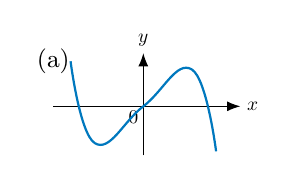
\begin{tikzpicture}[x=0.88cm, y=0.52cm, >=Latex]
    \node[font=\small] at (-1.3, 1.1) {(a)};
    \draw[->] (-1.3, 0) -- (1.4, 0) node[right, scale=0.7] {$x$};
    \draw[->] (0, -1.2) -- (0, 1.3) node[above, scale=0.7] {$y$};
    \node[scale=0.7, below left=-1pt] at (0,0) {$0$};
    \draw[curveblue, thick] plot[smooth, tension=0.75] coordinates {
      (-1.05, 1.1) (-0.7, -0.9) (0, 0) (0.7, 0.9) (1.05, -1.1)
    };
  \end{tikzpicture}\hfill
  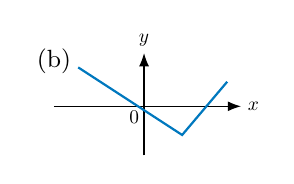
\begin{tikzpicture}[x=0.88cm, y=0.52cm, >=Latex]
    \node[font=\small] at (-1.3, 1.1) {(b)};
    \draw[->] (-1.3, 0) -- (1.4, 0) node[right, scale=0.7] {$x$};
    \draw[->] (0, -1.2) -- (0, 1.3) node[above, scale=0.7] {$y$};
    \node[scale=0.7, below left=-1pt] at (0,0) {$0$};
    \draw[curveblue, thick] (-0.95, 0.95) -- (0.55, -0.7) -- (1.2, 0.6);
  \end{tikzpicture}\par\vspace{2pt}

  % Hàng 2: (c) và (d)
  \noindent
  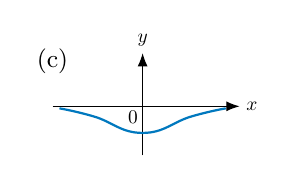
\begin{tikzpicture}[x=0.88cm, y=0.52cm, >=Latex]
    \node[font=\small] at (-1.3, 1.1) {(c)};
    \draw[->] (-1.3, 0) -- (1.4, 0) node[right, scale=0.7] {$x$};
    \draw[->] (0, -1.2) -- (0, 1.3) node[above, scale=0.7] {$y$};
    \node[scale=0.7, below left=-1pt] at (0,0) {$0$};
    \draw[curveblue, thick] plot[smooth, tension=0.8] coordinates {
      (-1.2, -0.05) (-0.7, -0.25) (0, -0.65) (0.7, -0.25) (1.2, -0.05)
    };
  \end{tikzpicture}\hfill
  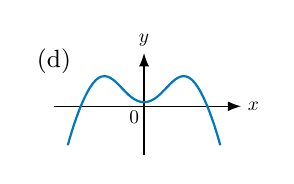
\begin{tikzpicture}[x=0.88cm, y=0.52cm, >=Latex]
    \node[font=\small] at (-1.3, 1.1) {(d)};
    \draw[->] (-1.3, 0) -- (1.4, 0) node[right, scale=0.7] {$x$};
    \draw[->] (0, -1.2) -- (0, 1.3) node[above, scale=0.7] {$y$};
    \node[scale=0.7, below left=-1pt] at (0,0) {$0$};
    \draw[curveblue, thick] plot[smooth, tension=0.75] coordinates {
      (-1.1, -0.95) (-0.65, 0.7) (0, 0.1) (0.65, 0.7) (1.1, -0.95)
    };
  \end{tikzpicture}\par\vspace{6pt}

  % Hàng 3: I và II
  \noindent
  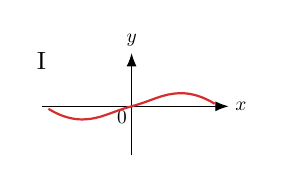
\begin{tikzpicture}[x=0.88cm, y=0.52cm, >=Latex]
    \node[font=\small] at (-1.3, 1.1) {I};
    \draw[->] (-1.3, 0) -- (1.4, 0) node[right, scale=0.7] {$x$};
    \draw[->] (0, -1.2) -- (0, 1.3) node[above, scale=0.7] {$y$};
    \node[scale=0.7, below left=-1pt] at (0,0) {$0$};
    \draw[curvered, thick] plot[smooth, tension=0.8] coordinates {
      (-1.2, -0.06) (-0.7, -0.32) (0, 0) (0.7, 0.32) (1.2, 0.06)
    };
  \end{tikzpicture}\hfill
  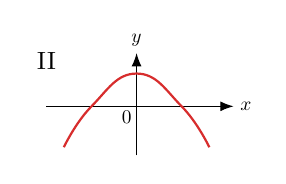
\begin{tikzpicture}[x=0.88cm, y=0.52cm, >=Latex]
    \node[font=\small] at (-1.3, 1.1) {II};
    \draw[->] (-1.3, 0) -- (1.4, 0) node[right, scale=0.7] {$x$};
    \draw[->] (0, -1.2) -- (0, 1.3) node[above, scale=0.7] {$y$};
    \node[scale=0.7, below left=-1pt] at (0,0) {$0$};
    \draw[curvered, thick] plot[smooth, tension=0.8] coordinates {
      (-1.05, -1.0) (-0.65, 0) (0, 0.8) (0.65, 0) (1.05, -1.0)
    };
  \end{tikzpicture}\par\vspace{2pt}

  % Hàng 4: III và IV
  \noindent
  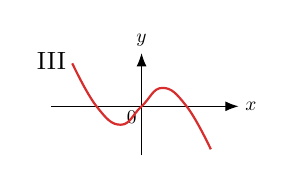
\begin{tikzpicture}[x=0.88cm, y=0.52cm, >=Latex]
    \node[font=\small] at (-1.3, 1.1) {III};
    \draw[->] (-1.3, 0) -- (1.4, 0) node[right, scale=0.7] {$x$};
    \draw[->] (0, -1.2) -- (0, 1.3) node[above, scale=0.7] {$y$};
    \node[scale=0.7, below left=-1pt] at (0,0) {$0$};
    \draw[curvered, thick] plot[smooth, tension=0.75] coordinates {
      (-1.0, 1.05) (-0.65, 0) (-0.3, -0.45) (0, 0) (0.3, 0.45) (0.65, 0) (1.0, -1.05)
    };
  \end{tikzpicture}\hfill
  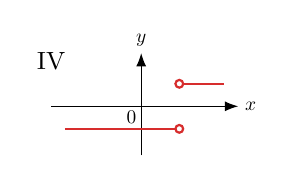
\begin{tikzpicture}[x=0.88cm, y=0.52cm, >=Latex]
    \node[font=\small] at (-1.3, 1.1) {IV};
    \draw[->] (-1.3, 0) -- (1.4, 0) node[right, scale=0.7] {$x$};
    \draw[->] (0, -1.2) -- (0, 1.3) node[above, scale=0.7] {$y$};
    \node[scale=0.7, below left=-1pt] at (0,0) {$0$};
    \draw[curvered, thick] (-1.1, -0.55) -- (0.5, -0.55);
    \draw[curvered, thick, fill=white] (0.55, -0.55) circle (1.4pt);
    \draw[curvered, thick] (0.6, 0.55) -- (1.2, 0.55);
    \draw[curvered, thick, fill=white] (0.55, 0.55) circle (1.4pt);
  \end{tikzpicture}\par\vspace{8pt}

  % Khối bài 4-11
  {\color{stewartblue}\textbf{4–11}}\quad Can hoặc vẽ lại đồ thị của hàm số $f$ đã cho. (Giả sử các trục tọa độ có cùng tỉ lệ.) Sau đó sử dụng phương pháp của Ví dụ 1 để phác thảo đồ thị của $f'$ ngay bên dưới nó.\par\vspace{6pt}

  % Hàng 5: 4 và 5
  \noindent
  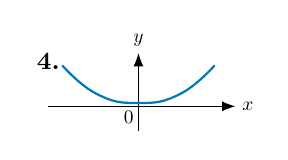
\begin{tikzpicture}[x=0.88cm, y=0.52cm, >=Latex]
    \node[font=\small\bfseries] at (-1.3, 1.1) {4.};
    \draw[->] (-1.3, 0) -- (1.4, 0) node[right, scale=0.7] {$x$};
    \draw[->] (0, -0.6) -- (0, 1.3) node[above, scale=0.7] {$y$};
    \node[scale=0.7, below left=-1pt] at (0,0) {$0$};
    \draw[curveblue, thick] plot[smooth, tension=0.8] coordinates {
      (-1.1, 1.0) (-0.6, 0.3) (0, 0.08) (0.6, 0.3) (1.1, 1.0)
    };
  \end{tikzpicture}\hfill
  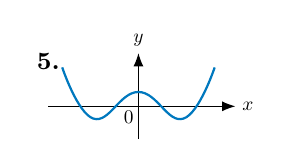
\begin{tikzpicture}[x=0.88cm, y=0.52cm, >=Latex]
    \node[font=\small\bfseries] at (-1.3, 1.1) {5.};
    \draw[->] (-1.3, 0) -- (1.4, 0) node[right, scale=0.7] {$x$};
    \draw[->] (0, -0.8) -- (0, 1.3) node[above, scale=0.7] {$y$};
    \node[scale=0.7, below left=-1pt] at (0,0) {$0$};
    \draw[curveblue, thick] plot[smooth, tension=0.75] coordinates {
      (-1.1, 0.95) (-0.65, -0.3) (0, 0.35) (0.65, -0.3) (1.1, 0.95)
    };
  \end{tikzpicture}\par\vspace{4pt}

  % Hàng 6: 6 và 7
  \noindent
  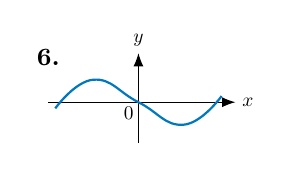
\begin{tikzpicture}[x=0.88cm, y=0.52cm, >=Latex]
    \node[font=\small\bfseries] at (-1.3, 1.1) {6.};
    \draw[->] (-1.3, 0) -- (1.4, 0) node[right, scale=0.7] {$x$};
    \draw[->] (0, -1.0) -- (0, 1.2) node[above, scale=0.7] {$y$};
    \node[scale=0.7, below left=-1pt] at (0,0) {$0$};
    \draw[curveblue, thick] plot[smooth, tension=0.8] coordinates {
      (-1.2, -0.15) (-0.65, 0.55) (0, 0) (0.65, -0.55) (1.2, 0.15)
    };
  \end{tikzpicture}\hfill
  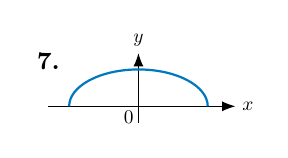
\begin{tikzpicture}[x=0.88cm, y=0.52cm, >=Latex]
    \node[font=\small\bfseries] at (-1.3, 1.1) {7.};
    \draw[->] (-1.3, 0) -- (1.4, 0) node[right, scale=0.7] {$x$};
    \draw[->] (0, -0.4) -- (0, 1.3) node[above, scale=0.7] {$y$};
    \node[scale=0.7, below left=-1pt] at (0,0) {$0$};
    \draw[curveblue, thick] (-1.0, 0) arc[start angle=180, end angle=0, x radius=1.0, y radius=0.9];
  \end{tikzpicture}
\end{minipage}\hfill
% ==================== CỘT PHẢI ====================
\begin{minipage}[t]{0.48\textwidth}
  % Hàng 7: 8 và 9
  \noindent
  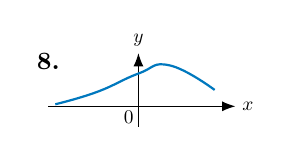
\begin{tikzpicture}[x=0.88cm, y=0.52cm, >=Latex]
    \node[font=\small\bfseries] at (-1.3, 1.1) {8.};
    \draw[->] (-1.3, 0) -- (1.4, 0) node[right, scale=0.7] {$x$};
    \draw[->] (0, -0.5) -- (0, 1.3) node[above, scale=0.7] {$y$};
    \node[scale=0.7, below left=-1pt] at (0,0) {$0$};
    \draw[curveblue, thick] plot[smooth, tension=0.8] coordinates {
      (-1.2, 0.05) (-0.6, 0.35) (0, 0.8) (0.45, 1.0) (1.1, 0.4)
    };
  \end{tikzpicture}\hfill
  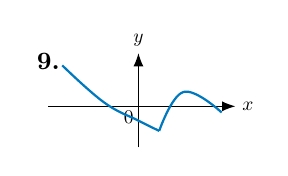
\begin{tikzpicture}[x=0.88cm, y=0.52cm, >=Latex]
    \node[font=\small\bfseries] at (-1.3, 1.1) {9.};
    \draw[->] (-1.3, 0) -- (1.4, 0) node[right, scale=0.7] {$x$};
    \draw[->] (0, -1.0) -- (0, 1.3) node[above, scale=0.7] {$y$};
    \node[scale=0.7, below left=-1pt] at (0,0) {$0$};
    \draw[curveblue, thick] plot[smooth, tension=0.7] coordinates {(-1.1, 1.0) (-0.5, 0.1) (0, -0.35) (0.3, -0.6)};
    \draw[curveblue, thick] plot[smooth, tension=0.7] coordinates {(0.3, -0.6) (0.65, 0.35) (1.2, -0.15)};
  \end{tikzpicture}\par\vspace{4pt}

  % Hàng 8: 10 và 11
  \noindent
  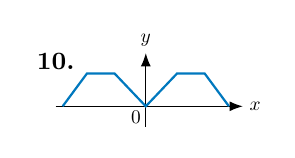
\begin{tikzpicture}[x=0.88cm, y=0.52cm, >=Latex]
    \node[font=\small\bfseries] at (-1.3, 1.1) {10.};
    \draw[->] (-1.3, 0) -- (1.4, 0) node[right, scale=0.7] {$x$};
    \draw[->] (0, -0.5) -- (0, 1.3) node[above, scale=0.7] {$y$};
    \node[scale=0.7, below left=-1pt] at (0,0) {$0$};
    \draw[curveblue, thick] (-1.2, 0) -- (-0.85, 0.8) -- (-0.45, 0.8) -- (0, 0) -- (0.45, 0.8) -- (0.85, 0.8) -- (1.2, 0);
  \end{tikzpicture}\hfill
  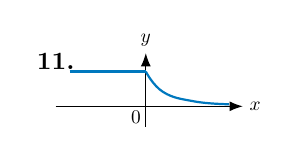
\begin{tikzpicture}[x=0.88cm, y=0.52cm, >=Latex]
    \node[font=\small\bfseries] at (-1.3, 1.1) {11.};
    \draw[->] (-1.3, 0) -- (1.4, 0) node[right, scale=0.7] {$x$};
    \draw[->] (0, -0.5) -- (0, 1.3) node[above, scale=0.7] {$y$};
    \node[scale=0.7, below left=-1pt] at (0,0) {$0$};
    \draw[curveblue, thick] (-1.1, 0.85) -- (0, 0.85);
    \draw[curveblue, thick] plot[smooth, tension=0.75] coordinates {(0, 0.85) (0.25, 0.35) (0.7, 0.12) (1.2, 0.05)};
  \end{tikzpicture}\par\vspace{8pt}

  % Bài 12
  \textbf{12.} Hình bên biểu diễn đồ thị hàm số kích thước quần thể $P(t)$ của các tế bào nấm men trong một mẻ cấy phòng thí nghiệm. Sử dụng phương pháp của Ví dụ 1 để vẽ đồ thị đạo hàm $P'(t)$. Đồ thị của $P'$ cho ta biết điều gì về quần thể nấm men?\par\vspace{4pt}
  \begin{center}
    \begin{tikzpicture}[x=0.33cm, y=0.0035cm, >=Latex]
      \draw[->] (0,0) -- (18, 0) node[right, scale=0.75] {$t\text{ (giờ)}$};
      \draw[->] (0,0) -- (0, 720) node[above, scale=0.75] {$P$};
      \node[scale=0.7, anchor=west] at (0.2, 690) {(tế bào nấm men)};
      \node[scale=0.7, below left=-1pt] at (0,0) {$0$};
      \foreach \x in {5, 10, 15} {
        \draw (\x, 0) -- (\x, -18) node[below, scale=0.7] {$\x$};
      }
      \draw (0, 500) -- (-0.35, 500) node[left, scale=0.7] {$500$};
      \draw[curveblue, thick] plot[smooth, tension=0.8] coordinates {
        (0, 45) (3, 90) (6, 210) (8, 370) (10, 500) (12, 580) (15, 625) (17, 635)
      };
    \end{tikzpicture}
  \end{center}\vspace{2pt}

  % Bài 13
  \textbf{13.} Một pin sạc được cắm vào bộ sạc. Đồ thị cho thấy $C(t)$, tỉ lệ phần trăm dung lượng đầy mà pin đạt được như một hàm theo thời gian trôi qua $t$ (tính bằng giờ).
  \begin{enumerate}[label=(\alph*), leftmargin=1.5em, itemsep=0pt, topsep=1pt]
    \item Ý nghĩa của đạo hàm $C'(t)$ là gì?
    \item Phác thảo đồ thị của $C'(t)$. Đồ thị đó cho bạn biết điều gì?
  \end{enumerate}
  \begin{center}
    \begin{tikzpicture}[x=0.36cm, y=0.021cm, >=Latex]
      \draw[->] (0,0) -- (13.5, 0) node[right, scale=0.75] {$t\text{ (giờ)}$};
      \draw[->] (0,0) -- (0, 115) node[above, scale=0.75] {$C$};
      \node[scale=0.68, align=center, rotate=90] at (-2.3, 58) {Phần trăm dung lượng đầy};
      \node[scale=0.7, below left=-1pt] at (0,0) {$0$};
      \foreach \x in {2, 4, 6, 8, 10, 12} {
        \draw (\x, 0) -- (\x, -2.5) node[below, scale=0.7] {$\x$};
      }
      \foreach \y in {20, 40, 60, 80, 100} {
        \draw (0, \y) -- (-0.3, \y) node[left, scale=0.7] {$\y$};
      }
      \draw[curveblue, thick] plot[smooth, tension=0.8] coordinates {
        (0, 0) (2, 45) (4, 71) (6, 86) (8, 93) (10, 97) (12, 99)
      };
    \end{tikzpicture}
  \end{center}\vspace{2pt}

  % Bài 14
  \textbf{14.} Đồ thị (từ Bộ Năng lượng Hoa Kỳ) cho thấy tốc độ lái xe ảnh hưởng như thế nào đến mức tiêu hao nhiên liệu. Hiệu quả nhiên liệu $F$ được đo bằng dặm trên gallon và tốc độ $v$ được đo bằng dặm trên giờ.
  \begin{enumerate}[label=(\alph*), leftmargin=1.5em, itemsep=0pt, topsep=1pt]
    \item Ý nghĩa của đạo hàm $F'(v)$ là gì?
    \item Phác thảo đồ thị của $F'(v)$.
  \end{enumerate}
\end{minipage}

\vspace*{\fill}
\noindent{\tiny\color{gray} Copyright 2021 Cengage Learning. All Rights Reserved. May not be copied, scanned, or duplicated, in whole or in part. WCN 02-200-203}

\end{document}